% Created by tikzDevice version 0.12.6 on 2024-11-11 08:51:27
% !TEX encoding = UTF-8 Unicode
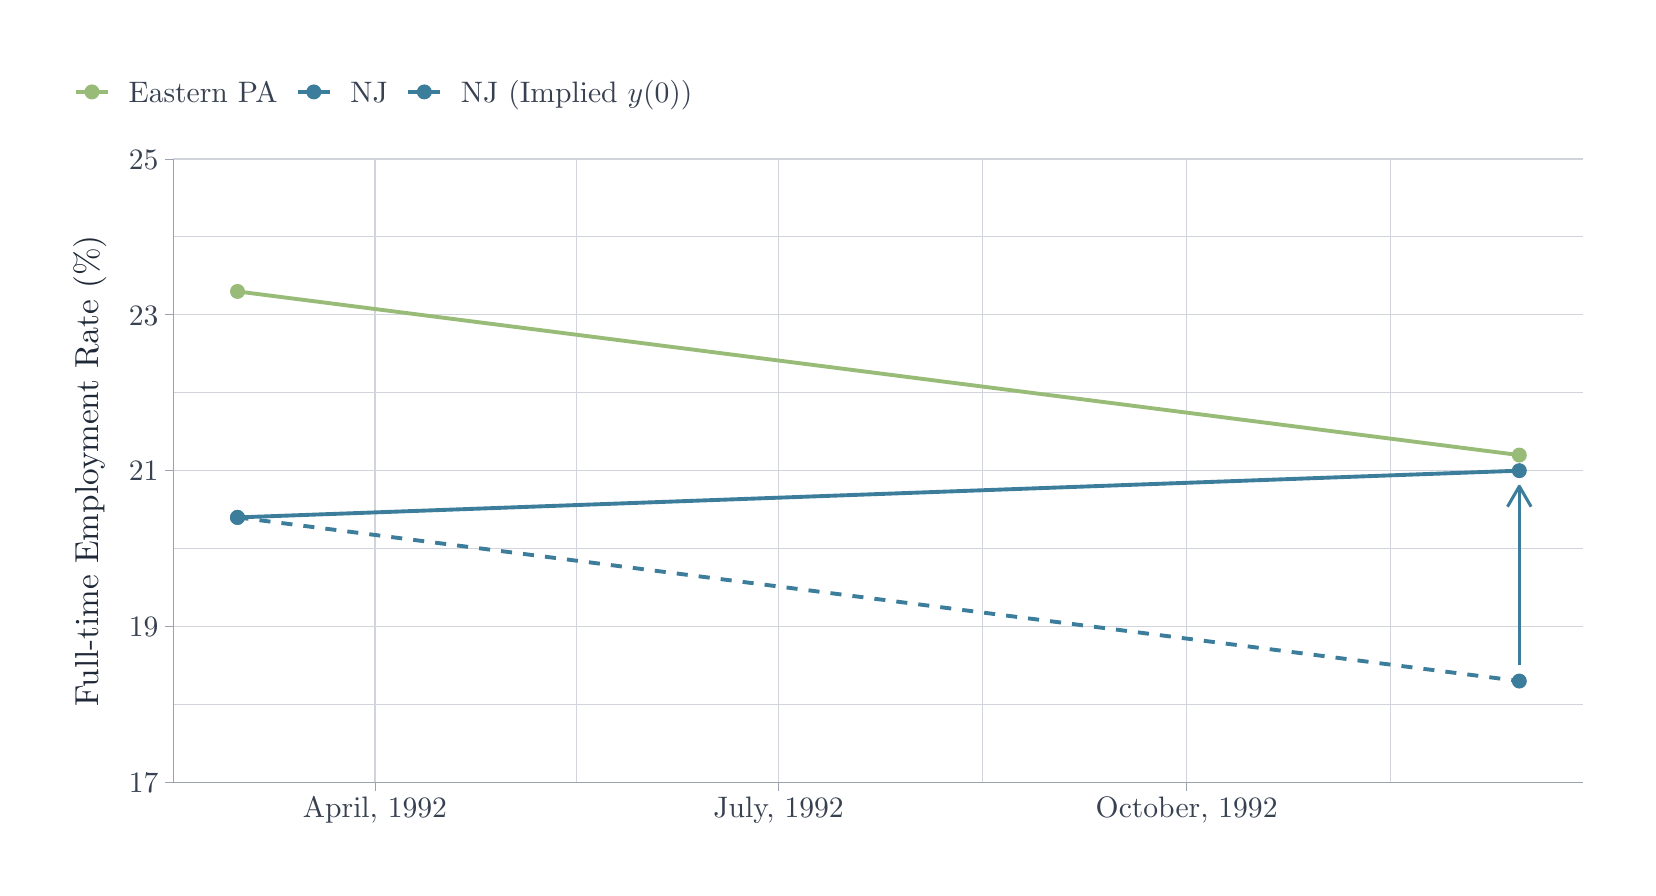
\begin{tikzpicture}[x=1pt,y=1pt]
\definecolor{fillColor}{RGB}{255,255,255}
\path[use as bounding box,fill=fillColor] (0,0) rectangle (578.16,303.53);
\begin{scope}
\path[clip] (  0.00,  0.00) rectangle (578.16,303.53);
\definecolor{drawColor}{RGB}{255,255,255}

\path[draw=drawColor,line width= 0.6pt,line join=round,line cap=round,fill=fillColor] (  0.00,  0.00) rectangle (578.16,303.53);
\end{scope}
\begin{scope}
\path[clip] ( 52.66, 30.82) rectangle (562.16,256.08);
\definecolor{drawColor}{RGB}{255,255,255}
\definecolor{fillColor}{RGB}{255,255,255}

\path[draw=drawColor,line width= 0.6pt,line join=round,line cap=round,fill=fillColor] ( 52.66, 30.82) rectangle (562.16,256.08);
\definecolor{drawColor}{RGB}{209,213,219}

\path[draw=drawColor,line width= 0.4pt,line join=round] ( 52.66, 58.98) --
	(562.16, 58.98);

\path[draw=drawColor,line width= 0.4pt,line join=round] ( 52.66,115.29) --
	(562.16,115.29);

\path[draw=drawColor,line width= 0.4pt,line join=round] ( 52.66,171.61) --
	(562.16,171.61);

\path[draw=drawColor,line width= 0.4pt,line join=round] ( 52.66,227.92) --
	(562.16,227.92);

\path[draw=drawColor,line width= 0.4pt,line join=round] (198.43, 30.82) --
	(198.43,256.08);

\path[draw=drawColor,line width= 0.4pt,line join=round] (345.08, 30.82) --
	(345.08,256.08);

\path[draw=drawColor,line width= 0.4pt,line join=round] (492.52, 30.82) --
	(492.52,256.08);

\path[draw=drawColor,line width= 0.4pt,line join=round] ( 52.66, 30.82) --
	(562.16, 30.82);

\path[draw=drawColor,line width= 0.4pt,line join=round] ( 52.66, 87.14) --
	(562.16, 87.14);

\path[draw=drawColor,line width= 0.4pt,line join=round] ( 52.66,143.45) --
	(562.16,143.45);

\path[draw=drawColor,line width= 0.4pt,line join=round] ( 52.66,199.77) --
	(562.16,199.77);

\path[draw=drawColor,line width= 0.4pt,line join=round] ( 52.66,256.08) --
	(562.16,256.08);

\path[draw=drawColor,line width= 0.4pt,line join=round] (125.51, 30.82) --
	(125.51,256.08);

\path[draw=drawColor,line width= 0.4pt,line join=round] (271.35, 30.82) --
	(271.35,256.08);

\path[draw=drawColor,line width= 0.4pt,line join=round] (418.80, 30.82) --
	(418.80,256.08);
\definecolor{drawColor}{RGB}{59,125,155}
\definecolor{fillColor}{RGB}{59,125,155}

\path[draw=drawColor,line width= 0.4pt,line join=round,line cap=round,fill=fillColor] ( 75.82,126.56) circle (  2.50);

\path[draw=drawColor,line width= 0.4pt,line join=round,line cap=round,fill=fillColor] (539.00,143.45) circle (  2.50);

\path[draw=drawColor,line width= 0.4pt,line join=round,line cap=round,fill=fillColor] ( 75.82,126.56) circle (  2.50);

\path[draw=drawColor,line width= 0.4pt,line join=round,line cap=round,fill=fillColor] (539.00, 67.43) circle (  2.50);
\definecolor{drawColor}{RGB}{152,188,120}
\definecolor{fillColor}{RGB}{152,188,120}

\path[draw=drawColor,line width= 0.4pt,line join=round,line cap=round,fill=fillColor] ( 75.82,208.21) circle (  2.50);

\path[draw=drawColor,line width= 0.4pt,line join=round,line cap=round,fill=fillColor] (539.00,149.08) circle (  2.50);

\path[draw=drawColor,line width= 1.4pt,line join=round] ( 75.82,208.21) --
	(539.00,149.08);
\definecolor{drawColor}{RGB}{59,125,155}

\path[draw=drawColor,line width= 1.4pt,line join=round] ( 75.82,126.56) --
	(539.00,143.45);

\path[draw=drawColor,line width= 1.4pt,dash pattern=on 4pt off 4pt ,line join=round] ( 75.82,126.56) --
	(539.00, 67.43);

\path[draw=drawColor,line width= 1.1pt,line join=round] (539.00, 73.06) -- (539.00,137.82);

\path[draw=drawColor,line width= 1.1pt,line join=round] (543.27,130.43) --
	(539.00,137.82) --
	(534.73,130.43);
\end{scope}
\begin{scope}
\path[clip] (  0.00,  0.00) rectangle (578.16,303.53);
\definecolor{drawColor}{RGB}{156,163,175}

\path[draw=drawColor,line width= 0.3pt,line join=round] ( 52.66, 30.82) --
	( 52.66,256.08);
\end{scope}
\begin{scope}
\path[clip] (  0.00,  0.00) rectangle (578.16,303.53);
\definecolor{drawColor}{RGB}{55,65,81}

\node[text=drawColor,anchor=base east,inner sep=0pt, outer sep=0pt, scale=  1.07] at ( 47.26, 27.15) {17};

\node[text=drawColor,anchor=base east,inner sep=0pt, outer sep=0pt, scale=  1.07] at ( 47.26, 83.46) {19};

\node[text=drawColor,anchor=base east,inner sep=0pt, outer sep=0pt, scale=  1.07] at ( 47.26,139.78) {21};

\node[text=drawColor,anchor=base east,inner sep=0pt, outer sep=0pt, scale=  1.07] at ( 47.26,196.09) {23};

\node[text=drawColor,anchor=base east,inner sep=0pt, outer sep=0pt, scale=  1.07] at ( 47.26,252.41) {25};
\end{scope}
\begin{scope}
\path[clip] (  0.00,  0.00) rectangle (578.16,303.53);
\definecolor{drawColor}{RGB}{156,163,175}

\path[draw=drawColor,line width= 0.3pt,line join=round] ( 49.66, 30.82) --
	( 52.66, 30.82);

\path[draw=drawColor,line width= 0.3pt,line join=round] ( 49.66, 87.14) --
	( 52.66, 87.14);

\path[draw=drawColor,line width= 0.3pt,line join=round] ( 49.66,143.45) --
	( 52.66,143.45);

\path[draw=drawColor,line width= 0.3pt,line join=round] ( 49.66,199.77) --
	( 52.66,199.77);

\path[draw=drawColor,line width= 0.3pt,line join=round] ( 49.66,256.08) --
	( 52.66,256.08);
\end{scope}
\begin{scope}
\path[clip] (  0.00,  0.00) rectangle (578.16,303.53);
\definecolor{drawColor}{RGB}{156,163,175}

\path[draw=drawColor,line width= 0.3pt,line join=round] ( 52.66, 30.82) --
	(562.16, 30.82);
\end{scope}
\begin{scope}
\path[clip] (  0.00,  0.00) rectangle (578.16,303.53);
\definecolor{drawColor}{RGB}{156,163,175}

\path[draw=drawColor,line width= 0.3pt,line join=round] (125.51, 27.82) --
	(125.51, 30.82);

\path[draw=drawColor,line width= 0.3pt,line join=round] (271.35, 27.82) --
	(271.35, 30.82);

\path[draw=drawColor,line width= 0.3pt,line join=round] (418.80, 27.82) --
	(418.80, 30.82);
\end{scope}
\begin{scope}
\path[clip] (  0.00,  0.00) rectangle (578.16,303.53);
\definecolor{drawColor}{RGB}{55,65,81}

\node[text=drawColor,anchor=base,inner sep=0pt, outer sep=0pt, scale=  1.07] at (125.51, 18.07) {April, 1992};

\node[text=drawColor,anchor=base,inner sep=0pt, outer sep=0pt, scale=  1.07] at (271.35, 18.07) {July, 1992};

\node[text=drawColor,anchor=base,inner sep=0pt, outer sep=0pt, scale=  1.07] at (418.80, 18.07) {October, 1992};
\end{scope}
\begin{scope}
\path[clip] (  0.00,  0.00) rectangle (578.16,303.53);
\definecolor{drawColor}{RGB}{31,41,55}

\node[text=drawColor,rotate= 90.00,anchor=base,inner sep=0pt, outer sep=0pt, scale=  1.20] at ( 25.43,143.45) {Full-time Employment Rate (\%)};
\end{scope}
\begin{scope}
\path[clip] (  0.00,  0.00) rectangle (578.16,303.53);
\definecolor{drawColor}{RGB}{255,255,255}
\definecolor{fillColor}{RGB}{255,255,255}

\path[draw=drawColor,line width= 0.6pt,line join=round,line cap=round,fill=fillColor] ( 16.00,268.08) rectangle (239.97,287.53);
\end{scope}
\begin{scope}
\path[clip] (  0.00,  0.00) rectangle (578.16,303.53);
\definecolor{drawColor}{RGB}{255,255,255}
\definecolor{fillColor}{RGB}{255,255,255}

\path[draw=drawColor,line width= 0.6pt,line join=round,line cap=round,fill=fillColor] ( 16.00,273.08) rectangle ( 30.45,287.53);
\end{scope}
\begin{scope}
\path[clip] (  0.00,  0.00) rectangle (578.16,303.53);
\definecolor{drawColor}{RGB}{152,188,120}
\definecolor{fillColor}{RGB}{152,188,120}

\path[draw=drawColor,line width= 0.4pt,line join=round,line cap=round,fill=fillColor] ( 23.23,280.31) circle (  2.50);
\end{scope}
\begin{scope}
\path[clip] (  0.00,  0.00) rectangle (578.16,303.53);
\definecolor{drawColor}{RGB}{152,188,120}

\path[draw=drawColor,line width= 1.4pt,line join=round] ( 17.45,280.31) -- ( 29.01,280.31);
\end{scope}
\begin{scope}
\path[clip] (  0.00,  0.00) rectangle (578.16,303.53);
\definecolor{drawColor}{RGB}{255,255,255}
\definecolor{fillColor}{RGB}{255,255,255}

\path[draw=drawColor,line width= 0.6pt,line join=round,line cap=round,fill=fillColor] ( 96.18,273.08) rectangle (110.63,287.53);
\end{scope}
\begin{scope}
\path[clip] (  0.00,  0.00) rectangle (578.16,303.53);
\definecolor{drawColor}{RGB}{59,125,155}
\definecolor{fillColor}{RGB}{59,125,155}

\path[draw=drawColor,line width= 0.4pt,line join=round,line cap=round,fill=fillColor] (103.40,280.31) circle (  2.50);
\end{scope}
\begin{scope}
\path[clip] (  0.00,  0.00) rectangle (578.16,303.53);
\definecolor{drawColor}{RGB}{59,125,155}

\path[draw=drawColor,line width= 1.4pt,line join=round] ( 97.62,280.31) -- (109.18,280.31);
\end{scope}
\begin{scope}
\path[clip] (  0.00,  0.00) rectangle (578.16,303.53);
\definecolor{drawColor}{RGB}{255,255,255}
\definecolor{fillColor}{RGB}{255,255,255}

\path[draw=drawColor,line width= 0.6pt,line join=round,line cap=round,fill=fillColor] (136.11,273.08) rectangle (150.57,287.53);
\end{scope}
\begin{scope}
\path[clip] (  0.00,  0.00) rectangle (578.16,303.53);
\definecolor{drawColor}{RGB}{59,125,155}
\definecolor{fillColor}{RGB}{59,125,155}

\path[draw=drawColor,line width= 0.4pt,line join=round,line cap=round,fill=fillColor] (143.34,280.31) circle (  2.50);
\end{scope}
\begin{scope}
\path[clip] (  0.00,  0.00) rectangle (578.16,303.53);
\definecolor{drawColor}{RGB}{59,125,155}

\path[draw=drawColor,line width= 1.4pt,dash pattern=on 4pt off 4pt ,line join=round] (137.56,280.31) -- (149.12,280.31);
\end{scope}
\begin{scope}
\path[clip] (  0.00,  0.00) rectangle (578.16,303.53);
\definecolor{drawColor}{RGB}{55,65,81}

\node[text=drawColor,anchor=base west,inner sep=0pt, outer sep=0pt, scale=  1.07] at ( 36.45,276.63) {Eastern PA};
\end{scope}
\begin{scope}
\path[clip] (  0.00,  0.00) rectangle (578.16,303.53);
\definecolor{drawColor}{RGB}{55,65,81}

\node[text=drawColor,anchor=base west,inner sep=0pt, outer sep=0pt, scale=  1.07] at (116.63,276.63) {NJ};
\end{scope}
\begin{scope}
\path[clip] (  0.00,  0.00) rectangle (578.16,303.53);
\definecolor{drawColor}{RGB}{55,65,81}

\node[text=drawColor,anchor=base west,inner sep=0pt, outer sep=0pt, scale=  1.07] at (156.57,276.63) {NJ (Implied $y(0)$)};
\end{scope}
\end{tikzpicture}
